\documentclass[utf8]{beamer}
\usetheme{Madrid}

\usepackage{array}
\usepackage{graphicx}
\usepackage[T1]{fontenc}
\usepackage[croatian]{babel}
\usepackage{bm}
\usepackage{amsfonts}
\usepackage{amsmath}

\newcommand{\iteralpha}{\boldsymbol{\alpha}_i^{k}}
\newcolumntype{L}[1]{>{\raggedright\let\newline\\\arraybackslash\hspace{0pt}}m{#1}}

\pdfmapfile{+sansmathaccent.map}

\graphicspath{{"grafika/"}}

\title[Primjena SVM-a za analizu sentimenta]
{Primjena stroja s potpornim vektorima za analizu sentimenta korisničkih recenzija}

\subtitle{Završni rad br. 5179}

\author{Dominik Stanojević}

\institute[FER]
{Sveučilište u Zagrebu, Fakultet elektrotehnike i računarstva}

\logo{
\includegraphics[height=1.5cm]{fer.png}}

\date{\today}

\begin{document}

\begin{frame}
\titlepage
\end{frame}
    
\begin{frame}
\frametitle{Sažetak}
\tableofcontents
\end{frame}
    
\section{Stroj s potpornim vektorima}
    
\subsection{Interpretacija modela}

\begin{frame}
\frametitle{Stroj s potpornim vektorima}
\begin{itemize}
\item Binarni klasifikator - primjerku $\mathbf{x}$ pridružena oznaka razreda $y \in \{-1, 1\}$
\item Linearni klasifikator
\end{itemize}
\begin{figure}
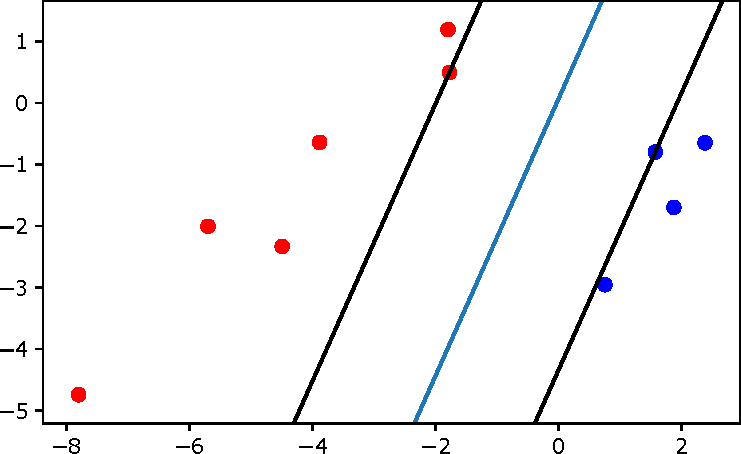
\includegraphics[scale=0.65]{support.pdf}
\caption{SVM kao klasifikator}
\end{figure}
\end{frame}	    

\begin{frame}
\frametitle{Hiperravnina}
Neka je zadan vektorski prostor $\textit{X}$ dimenzije $n$, primjerice $\mathbb{R}^n$.
Tada je \textbf{hiperravnina} definirana kao potprostor dimenzije $n-1$ unutar prostora $\textit{X}$.

\begin{block}{Jednadžba hiperravnine:}
$f(\mathbf{x})=b + \mathbf{w}^T\mathbf{x} = 0$
\end{block}

Svojstva hiperravnine:
\begin{enumerate}
  \item za svaku točku $T$ na hiperravnini vrijedi: $b = -\mathbf{w}^T\mathbf{x}$,
  \item jedinični vektor normale je zadan izrazom: $\mathbf{n} = \frac{\mathbf{w}}{\|\mathbf{w}\|}$,
  \item udaljenost točke $P$ od hiperravnine iznosi: $d = \frac{|f(\mathbf{x})|}{\|\mathbf{w}\|}$.
\end{enumerate}
\end{frame}

\begin{frame}
\frametitle{Razdvajajuća hiperravnina}
\begin{block}{Uvjet razdvajajuće hiperravnine:}
$y^{(i)} = sgn(b + \mathbf{w}^T\mathbf{x}^{(i)}), \forall i$
\end{block}
\begin{figure}
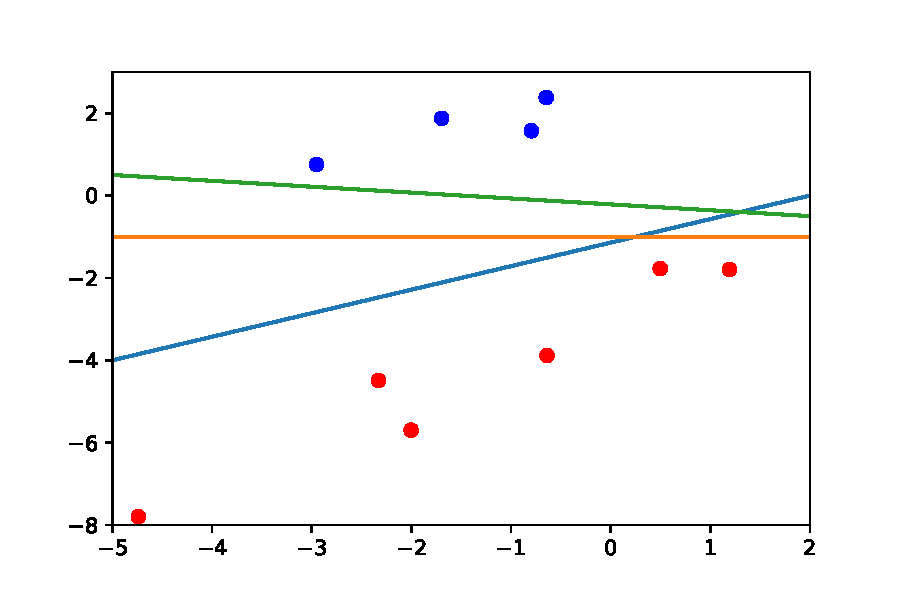
\includegraphics[scale=0.60]{hravnine.pdf}
\caption{Nekoliko razdvajajućih hiperravnina}
\end{figure}
\end{frame}

\begin{frame}
\frametitle{Margina razdvajajuće hiperravnine:}
\begin{block}{Margina hiperravnine:}
$\displaystyle M=\min_{i}\frac{y^{(i)}(b + \mathbf{w}^T\mathbf{x}^{(i)})}{\|\mathbf{w}\|}, 
y \in \{-1, 1\}.$
\end{block}

\begin{figure}
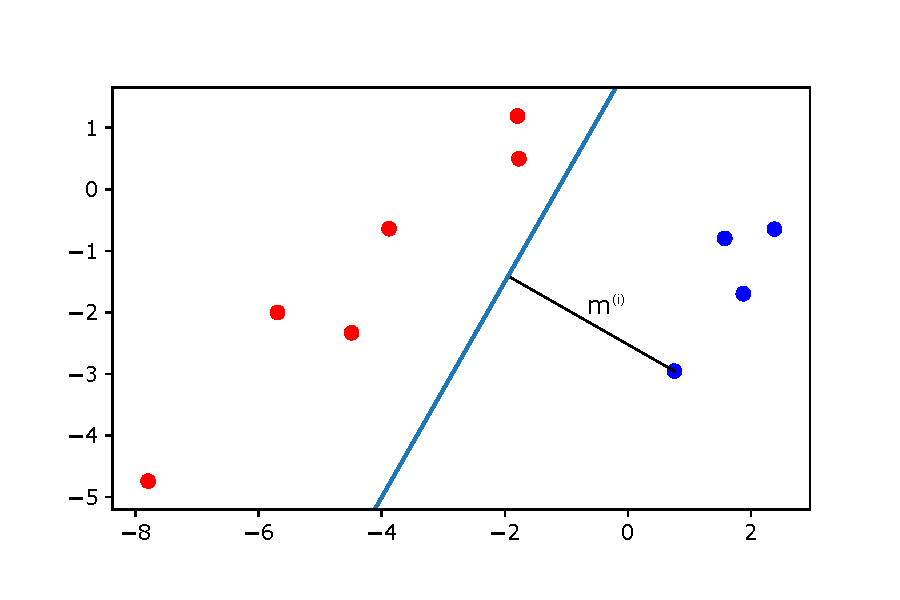
\includegraphics[scale=0.57]{distance.pdf}
\caption{Margina $i$-tog primjerka}
\end{figure}
\end{frame}

\begin{frame}
\frametitle{Optimalna razdvajajuća hiperravnina}
Inicijalni problem:
\begin{equation*}
\begin{aligned}
& \underset{\mathbf{w}, b}{\text{max}}
& & M \\
& \text{s obzirom na}
& & m^{(i)} \geq M, \; i = 1, \ldots, N
\end{aligned}
\end{equation*}

Nakon sređivanja:
\begin{equation*}
\begin{aligned}
& \underset{\mathbf{w}, b}{\text{min}}
& & \frac{1}{2}\|\mathbf{w}\|^2 \\
& \text{s obzirom na}
& & y^{(i)}(\mathbf{w}^T\mathbf{x}^{(i)} + b) \geq 1, \; i = 1, \ldots, N.
\end{aligned}
\end{equation*}
\end{frame}

\begin{frame}
\frametitle{Optimalna razdvajajuća hiperravnina}
\begin{figure}
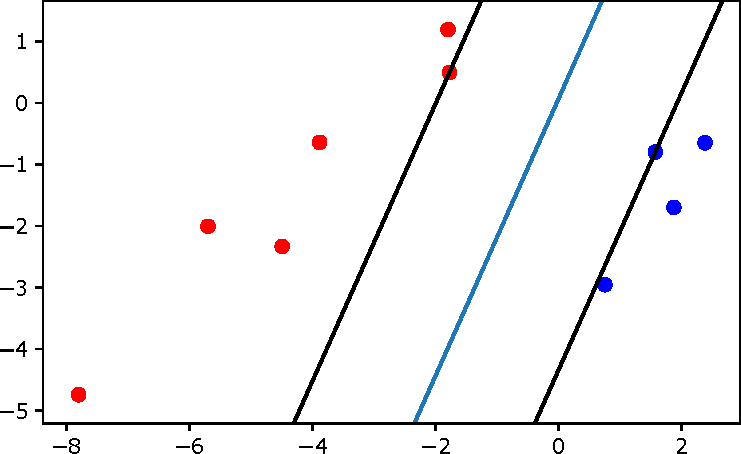
\includegraphics[scale=0.8]{support.pdf}
\caption{Maksimalna razdvajajuća hiperravnina}
\end{figure}
\end{frame}

\begin{frame}
\frametitle{Regularizacija}
\begin{figure}
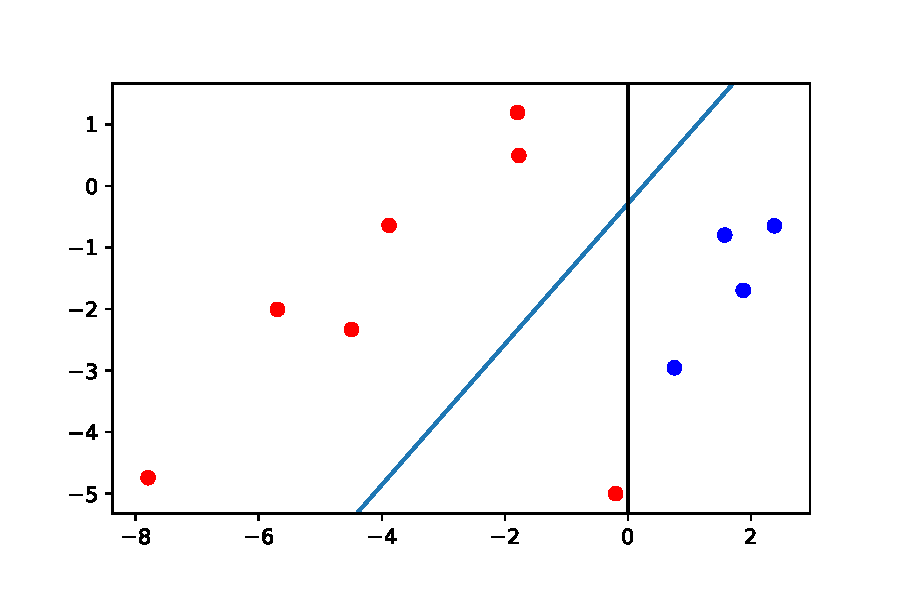
\includegraphics[scale=0.8]{outlier.pdf}
\caption{Utjecaj stršeće vrijednosti na odabir hiperravnine}
\end{figure}
\end{frame}

\begin{frame}
\frametitle{Regularizacija}
\alert{Regularizacija} je metoda kojom se sprječava pretreniranost modela koristeći funkciju kazne. 

\vspace{\baselineskip}

Najčešće funkcije kazne:
\begin{itemize}
\item L1-SVM: $\text{max}(1 - y^{(i)}\mathbf{w}^T\mathbf{x^{(i)}}, 0)$
\item L2-SVM: $\text{max}(1 - y^{(i)}\mathbf{w}^T\mathbf{x^{(i)}}, 0)^2$
\end{itemize}

\begin{block}{Redefiniranje optimizacijskog problema:}
\begin{equation*}
\begin{aligned}
& \underset{\mathbf{w}, b}{\text{min}}
& & \frac{1}{2}\|\mathbf{w}\|^2 + C\sum_{i=1}^{N} \xi_i\\
& \text{s obzirom na}
& & y^{(i)}(\mathbf{w}^T\mathbf{x}^{(i)} + b) \geq 1 - \xi_i, \; i = 1, \ldots, N \\
&&& \xi_i \geq 0, \; i = 1, \ldots, N.
\end{aligned}
\end{equation*}
\end{block}
\end{frame}

\subsection{Optimizacija SVM-a}

\begin{frame}
\frametitle{Primalni i dualni optimizacijski problem}
Optimizacijski problem:
\begin{equation*}
\begin{aligned}
& \underset{x}{\text{min}}
& & f(x)\\
& \text{s obzirom na}
& & g_i(x) \leq 0, \; i = 1, \ldots, m \\
&&& h_i(x) = 0, \; i = 1, \ldots, n.
\end{aligned}
\end{equation*}

Lagrangeova funkcija:
\begin{equation*}
\mathcal{L}(x, \alpha, \beta) = f(x) + \sum_{i=1}^{m}\alpha_ig_i(x) + \sum_{i=1}^{n}\beta_ih_i(x)
\end{equation*}

$\alpha_i, \beta_i$ nazivamo \alert{Lagrangeovim multiplikatorima}.
\end{frame}

\begin{frame}
\frametitle{Primalni i dualni optimizacijski problem}
Primarni problem:
\begin{equation*}
\begin{aligned}
p = \underset{x}{\text{min}}
\underset{\alpha, \beta, \alpha_i \geq 0}{\text{max}}
\mathcal{L}(x, \alpha, \beta).\\
\end{aligned}
\end{equation*}

Dualni problem:
\begin{equation*}
d = 
\underset{\alpha, \beta, \alpha_i \geq 0}{\text{max}} \underset{x}{\text{min}} \; \mathcal{L}(x, \alpha, \beta).
\end{equation*}

Interesantni slučaj:
\begin{equation*}
  p = d = \mathcal{L}(x, \alpha, \beta).
\end{equation*}
\end{frame}

\begin{frame}
\frametitle{Karush-Kuhn-Tucker uvjeti}
\begin{equation*}
  \frac{\partial \mathcal{L}(x, \alpha, \beta)}{\partial x_i} = 0, \; i = 1, \ldots, p
\end{equation*}
\begin{equation*}
  \frac{\partial \mathcal{L}(x, \alpha, \beta)}{\partial \beta_i} = 0, \; i = 1, \ldots, n
\end{equation*}
\begin{equation*}
  \alert{\alpha_ig_i(x) = 0}, \; i = 1, \ldots, m
\end{equation*}
\begin{equation*}
  g_i(x) \leq 0, \; i = 1, \ldots, m
\end{equation*}
\begin{equation*}
  \alpha_i \geq 0, \; i = 1, \ldots, m
\end{equation*}
\end{frame}

\begin{frame}
\frametitle{Optimizacija stroja s potpornim vektorima}
Lagrangeova funkcija:
\begin{align*}
  \mathcal{L}(\mathbf{w}, b, \xi,\alpha, \mu) 
  &= \frac{1}{2}\|\mathbf{w}\|^2 + C\sum_{i=1}^{N} \xi_i
  - \sum_{i=1}^{N} \alpha_i(y^{(i)}(\mathbf{w}^T\mathbf{x^{(i)}} + b) - (1 - \xi_i)) \\
  &- \sum_{i=1}^{N} \mu_i\xi_i.
\end{align*}

Deriviranjem po $\mathbf{w}, b, \xi$ i sređivanjem dolazi se do dualnog problema:
\begin{equation*}
\begin{aligned}
& \underset{\alpha}{\text{max}}
& & \sum_{i=1}^{N} \alpha_i - 
  \frac{1}{2}\sum_{i=1}^{N}\sum_{j=1}^{N} \alpha_i\alpha_jy^{(i)}y^{(j)}x^{(i)T}x^{(j)}\\
& \text{s obzirom na}
& & 0 \leq \alpha_i \leq C, \; i = 1, \ldots, N \\
&&& \sum_{i=1}^{N} \alpha_iy^{(i)} = 0.
\end{aligned}
\end{equation*}
\end{frame}

\begin{frame}
\frametitle{Potporni vektori}
Uvjet nejednakosti: 
\begin{equation*}
  g_i(\mathbf{w}, b) = - (y^{(i)}(\mathbf{w}^T\mathbf{x^{(i)}} + b) - (1 - \xi_i)) \leq 0.
\end{equation*}
U slučaju da vrijedi $g_i(\mathbf{w}, b) = 0$ za neki primjerak $(x^{(i)}, y^{(i)})$ tada
se taj primjerak naziva \alert{potpornim vektorom}. Za te primjerke pripadajući Lagrangeov multiplikator je različit od nule.

\begin{figure}
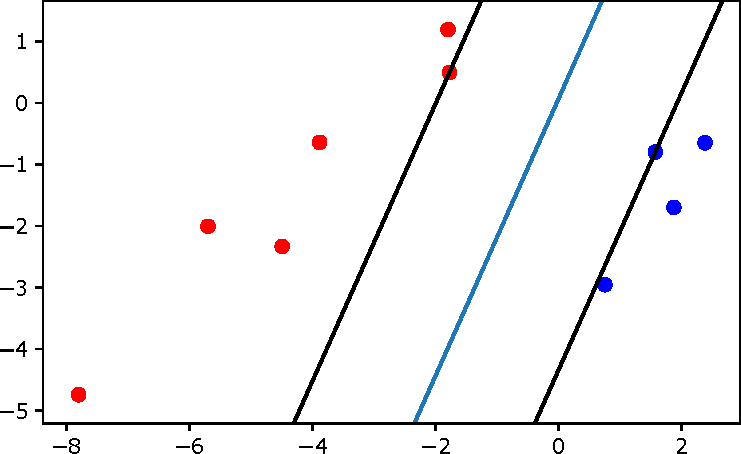
\includegraphics[scale=0.49]{support.pdf}
\caption{Potporni vektori}
\end{figure}
\end{frame}

\begin{frame}
\frametitle{Dualni koordinatni spust}
\begin{itemize}
\item Rješavanje dualnog optimizacijskog problema
\item U jednoj iteraciji osvježava se vrijednost samo jednog multiplikatora
\end{itemize}

\begin{figure}
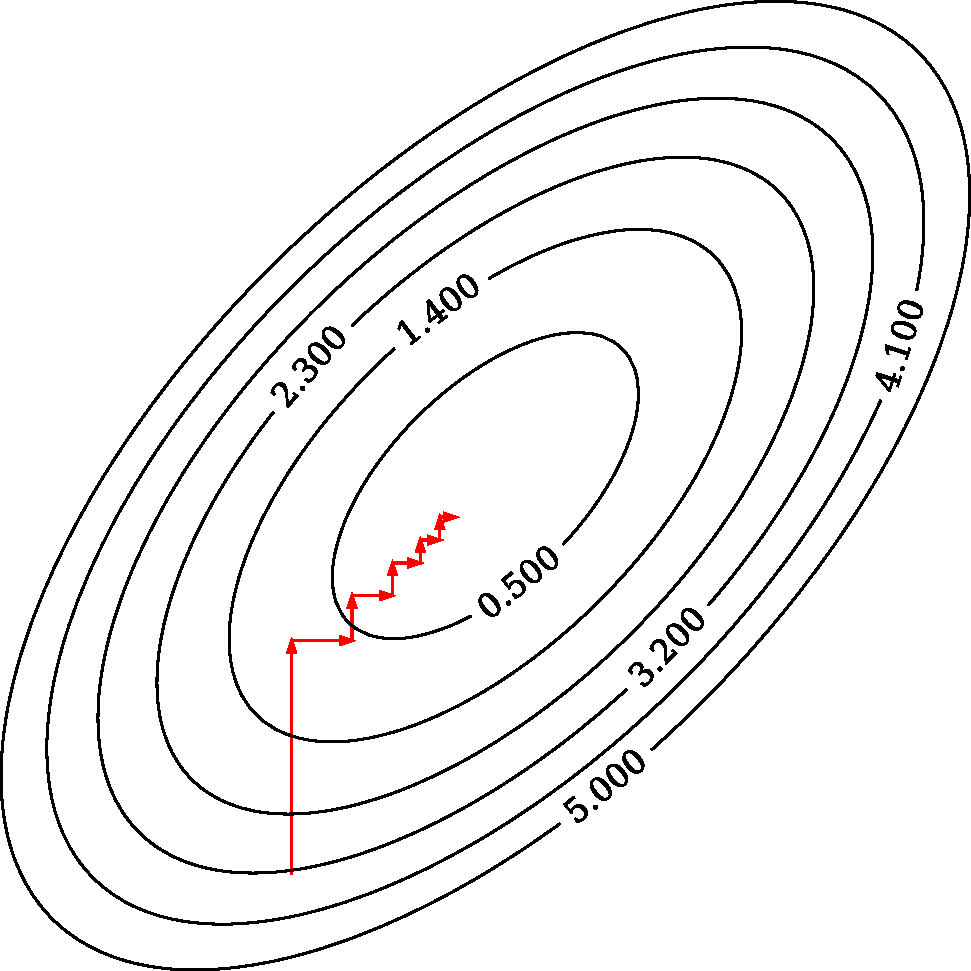
\includegraphics[scale=0.325]{dcd.pdf}
\caption{Koordinatni spust}
\end{figure}
\end{frame}

\begin{frame}
\frametitle{Dualni koordinatni spust}
Optimizacijski problem:
\begin{equation*}
\begin{aligned}
& \underset{\alpha}{\text{min}}
& & f(\boldsymbol{\alpha}) = \frac{1}{2}\boldsymbol{\alpha}^T\bar{\textbf{Q}}\boldsymbol{\alpha} 
- \textbf{e}^T\boldsymbol{\alpha}\\
& \text{s obzirom na}
& & 0 \leq \alpha_i \leq U, \; i = 1, \ldots, N.
\end{aligned}
\end{equation*}

Za L1-SVM vrijedi $U=C$ dok za L2-SVM vrijedi $U=\infty$. \\
Za matricu $\bar{\textbf{Q}}$ vrijedi izraz $\bar{\textbf{Q}} = \textbf{Q} + \textbf{D}$.\\
Elementi matrice $\textbf{Q}$ su $Q_{ij} = \alpha_i\alpha_jy^{(i)}y^{(j)}x^{(i)T}x^{(j)}$, dok je $\textbf{D}$ dijagonalna matrica.  
Za L1-SVM $\textbf{D}_{ii} = 0$, a za L2-SVM $D_{ii} = \frac{1}{2C}$.
\end{frame}

\begin{frame}
\frametitle{Dualni koordinatni spust}
Vanjska iteracija osvježava sve vrijednosti Lagrangeovih multiplikatora.
Unutarnja iteracija osvježava vrijednost jednog multiplikatora:
\begin{equation*} 
\begin{aligned}
& \underset{d}{\text{min}}
& & f(\iteralpha + d\textbf{e}_i) = \frac{1}{2}\bar{Q}_{ii}d^2 + 
\nabla_if(\iteralpha)d + C\\
& \text{s obzirom na}
& & 0 \leq \alpha_i + d \leq U, \; i = 1, \ldots, N
\end{aligned}
\end{equation*}

Osvježavanje vrijednosti multiplikatora:
\begin{equation*}
  \alpha_i^{k+1} = \text{min}(\text{max}(0, \alpha_i^{k} - \frac{\nabla_if(\iteralpha)}{\bar{Q}_{ii}}), U)
\end{equation*}

Direktno osvježavanje težina:
\begin{equation*} 
  \textbf{w} = \textbf{w} +  (\alpha_i^{k + 1} - \alpha_i^{k}) y^{(i)}\textbf{x}^{(i)}
\end{equation*}
\end{frame}

\subsection{Proširenje modela}

\begin{frame}
\frametitle{Jezgreni trikovi}
Klasifikacija primjerka koristeći Lagrangeove multiplikatore:
\begin{equation*}
  \hat{y} = sgn(\sum_{i=1}^{N} \alpha_iy^{(i)}\langle \phi(x), \phi(x^{(i)}) \rangle
  + b).
\end{equation*}

Zamjena umnoška s \alert{jezgrenom funkcijom} $K(x, x')$. Primjer:
\begin{equation*}
  K(\mathbf{x}, \mathbf{x}') = \text{exp}(- \frac{\|\mathbf{x} - \mathbf{x}'\|}{2\sigma^2})
\end{equation*}
\end{frame}

\begin{frame}
\frametitle{Jezgreni trik}
\begin{figure}
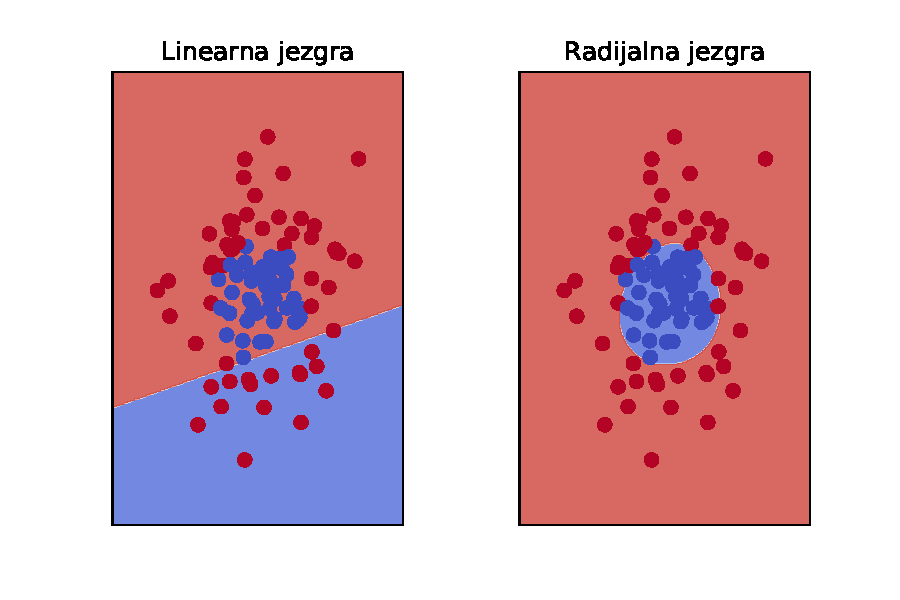
\includegraphics[scale=0.75]{kernel.pdf}
\caption{Klasifikacija podataka bez jezgrenog trika i s RBF}
\label{fig:kernel}
\end{figure}
\end{frame}

\begin{frame}
\frametitle{Višerazredna klasifikacija}
\begin{enumerate}
\item Jedan-naspram-ostalih - $N-1$ klasifikatora
\item Jedan-naspram-jedan - $\frac{N(N - 1)}{2}$ klasifikatora
\end{enumerate}
\end{frame}

\begin{frame}
\frametitle{Primjena SVM-a na regresijske probleme}

Optimizacijska funkcija:
\begin{equation*}
  f(\mathbf{w}, b) = \frac{1}{2}\|\mathbf{w}\|^2 + 
  C\sum_{i=1}^{N}(\xi_i^+ + \xi_i^-)
\end{equation*}

Uz uvjete:
\begin{equation*}
y^{(i)} - (\mathbf{w}^T\mathbf{x}^{(i)} + b) \leq \epsilon + \xi_i^+, \forall i 
\end{equation*}
\begin{equation*}
\mathbf{w}^T\mathbf{x}^{(i)} + b - y^{(i)} \leq \epsilon + \xi_i^-, \forall i
\end{equation*}

Postupak pretvorbe u dualni problem jednak kao i slučaju klasifikacije.
\end{frame}

\section{Analiza sentimenta}

\subsection{Ideja}
\begin{frame}
\frametitle{Definicija}
Analiza sentimenta (engl. \textit{Sentiment Analysis}) je područje posvećeno 
prikupljanju, obradi i analizi subjektivnih informacija, posebice stavova. \\~\\

Objektivna rečenica: \textit{"Danas je sunčano."} \\
Subjektivna rečenica: \textit{"Volim sunčan dan."} \\~\\

Uređena petorka: $(objekt, karakteristika, izvor, sentiment, vrijeme)$
\end{frame}

\begin{frame}
\frametitle{Primjer analiziranog teksta}
{\it
Užasan operacijski sustav. 
Osim osnovnih alata, upakiran je i s gomilu programa koji samo usporavaju rad sustava.
Nadam se da korisnici nisu ljubitelji privatnosti jer ju s ovim operacijskim sustavom
sigurno neće imati. 
Jedina pozitivna opcija je uvođenje radnih sati tako da me sustav rjeđe maltretira s 
ponovnim pokretanjem.
Savjet: potražite alternativu.
} Marko, 2016.

\begin{center}
(Operacijski sustav, "općenito", Marko, negativan, 2016.)\\
(Operacijski sustav, programski paket, Marko, negativan, 2016.)\\
(Operacijski sustav, razina privatnosti, Marko, negativan, 2016.)\\
(Operacijski sustav, vrijeme osvježavanja sustava, Marko, pozitivan, 2016.) \\
\end{center}
\end{frame}

\begin{frame}
\frametitle{Tipovi mišljenja}
\begin{itemize}
\item \textbf{Regularno mišljenje} - \textit{Volim kolače.}
\item \textbf{Komparativno mišljenje} - \textit{"Iako volim voćne kolače, draži su mi čokoladni."}
\item \textbf{Eksplicitno mišljenje} - \textit{Volim kolače.}
\item \textbf{Implicitno mišljenje} - \textit{"Baterija na mobitelu ne traje dovoljno dugo."}.
\end{itemize}
\end{frame}

\begin{frame}
\frametitle{Razine analize sentimenta}
\begin{enumerate}
\item Analiza na razini dokumenta
\item Analiza sentimenta na razini rečenica
\item Analiza sentimenta na razini karakteristika
\end{enumerate}
\end{frame}

\begin{frame}
\frametitle{Analiza sentimenta na razini dokumenta}

Cilj analize na razini dokumenta je pronaći sentiment osnovne informacijske jedinice, u ovom slučaju cijelog dokumenta. \\~\\

Formalno: $(\text{\_}, \text{"općenito"}, \text{\_}, s, \text{\_})$ \\~\\

Značajke:
\begin{itemize}
\item Subjektivne riječi i izrazi
\item Frekvencija izraza
\item Negacija
\end{itemize}
\end{frame}

\begin{frame}
\frametitle{Problemi prilikom analize sentimenta}
\begin{itemize}
\item Dvoznačnost
\item Nositelji sentimenta i implicitne rečenice
\item Sarkazam
\item Spam
\end{itemize}
\end{frame}

\subsection{Vektorizacija teksta}
\begin{frame}
\frametitle{Vektorizacija teksta}
Pretvorba dokumenta u vektor realnih brojeva - razumljivo SVM-u. \\~\\

Koraci:
\begin{enumerate}
\item Leksička analiza
\item Lematizacija
\item Izbacivanje zaustavnih riječi i interpunkcijskih znakova
\item Izgradnja N-grama
\item Izvlačenje značajki teksta
\end{enumerate}
\end{frame}

\begin{frame}
\frametitle{Leksička analiza}
\textbf{Leksička analiza} ili tokenizacija je postupak razdvajanja prepoznatljivih riječi, fraza i simbola. Jedna leksička jedinica zove se leksem. Leksičkom analizom tekst se pretvara u slijed leksema.

\begin{itemize}
\item Obrada HTML i XML oznaka - brisanje, posebni slučajevi (\textit{<strong>}, \textit{<b>}, ...)
\item Odvajanje leksema - razmaci, emotikoni, telefonski brojevi...
\item Negacija - prefiks NEG\_
\end{itemize}

\textit{"Ovo nije pozitivna rečenica :(."} $\Longrightarrow$
[\textit{Ovo}, \textit{NEG\_pozitivna}, \textit{NEG\_rečenica}, :(,  .]
\end{frame}

\begin{frame}
\frametitle{Lematizacija}
Postupak svođenja riječi na kanonski oblik. \\~\\

Primjer: \textit{najlošiji} $\Longrightarrow$ \textit{loš} \\~\\

Problemi: Agresivnost, gubitak intenziteta
\end{frame}

\begin{frame}
\frametitle{N-grami}

N-grami su izrazi koji se sastoje od $n$ slijednih leksema. \\~\\

Primjer: \textit{"Njegov savjet uzeo sam sa zrnom soli."}
\begin{itemize}
\item Unigrami (1-gram): [\textit{savjet}, \textit{uzeti}, \textit{zrno}, \textit{sol}]
\item Bigrami (2-gram): [\textit{savjet uzeti}, \textit{uzeti zrno}, 
\textit{zrno soli}]
\end{itemize}
\end{frame}

\begin{frame}
\frametitle{Izvlačenje značajki teksta}

Metode temeljne na modelu zbirki značajki (engl. \textit{Bag of words}). \\~\\

Modeli:
\begin{itemize}
\item Binarni - pojavnost izraza
\item Frekvencijski - frekvencija pojavljivanja
\item Model TF-IDF - relevantnost izraza za pojedini dokument i odnos relevantnosti između dokumenata
\end{itemize}
\end{frame}

\begin{frame}
\frametitle{Primjer izvlačenja značajki}
\begin{enumerate}
\item \textit{"Ovo je jako pozitivna rečenica."}
\item \textit{"Ovo je jako, jako negativna rečenica."}
\end{enumerate}

Primjer za drugu rečenicu:
\begin{center}
\scalebox{0.95}{
    \begin{tabular}{| l | c | c | c | c | c | c |}
    \hline
    Model/Izraz & Ovo & je & jako & poztivna & rečenica & negativna \\ \hline
    Binarni & 1 & 1 & 1 & 0 & 1 & 1\\ \hline
    Frekvencijski & 1 & 1 & 2 & 0 & 1 & 1\\ \hline
    TF-IDF & 0.3338 & 0.3338 & 0.6676 & 0 & 0.3338 & 0.4691 \\
    \hline
    \end{tabular}}
\end{center}

\begin{equation*}
  \text{tfidf}(t, d) = \text{tf}(t, d)\text{idf}(t, D) = 
  (1 + \text{log}(1+ f_{t, d}))\text{log}(1 + \frac{N}{n_t})
\end{equation*}
\end{frame}

\section{Rezultati i demonstracija}

\begin{frame}
\frametitle{Analiza korisničkih recenzija}

Large Movie Dataset Review:
\begin{itemize}
\item Prikupljeno s internetske baze filmova IMDB, obrađeno od strane sveučilišta Stanford
\item Više od 50000 korisničkih recenzija filmova
\item Pozitivna/negativna klasifikacija
\item 25000 pozitivnih recenzija; 25000 negativnih recenzija
\item 25000 trening recenzija; 25000 test recenzija; dodatne neoznačene recenzije
\end{itemize}
\end{frame}

\begin{frame}
\frametitle{Komponente leksičkog analizatora}
\begin{table}
    \center
    \begin{tabular}{| l | l | l |}
    \hline
    Metoda & Negacija isljučena & Negacija uključena \\ \hline
    Bez lematizacije i steminga & 89.18\% & 89.44\% \\ \hline
    Lematizacija & 89.01\% & 89.29\% \\ \hline
    Steming & 88.9\% & 89.33\% \\
    \hline
    \end{tabular}
    \caption{Točnost klasifikacije recenzija u odnosu na komponente leksičkog analizatora}
\end{table}
\end{frame}

\begin{frame}
\frametitle{Model vektorizacije i dimenzionalnost}
\begin{figure}
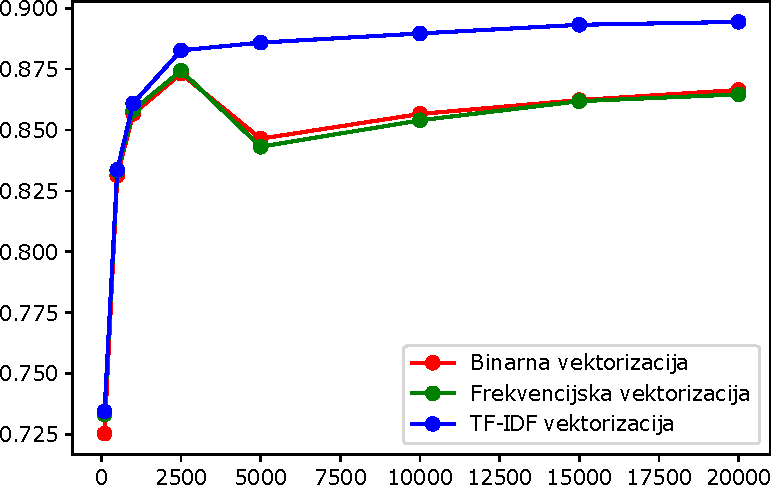
\includegraphics[scale=0.7]{vec_model.pdf}
\caption{Točnost klasifikacije u odnosu na model vektorizacije i dimenziju vektora značajki}
\end{figure}
\end{frame}

\begin{frame}
\frametitle{Izbor n-grama}
\begin{figure}
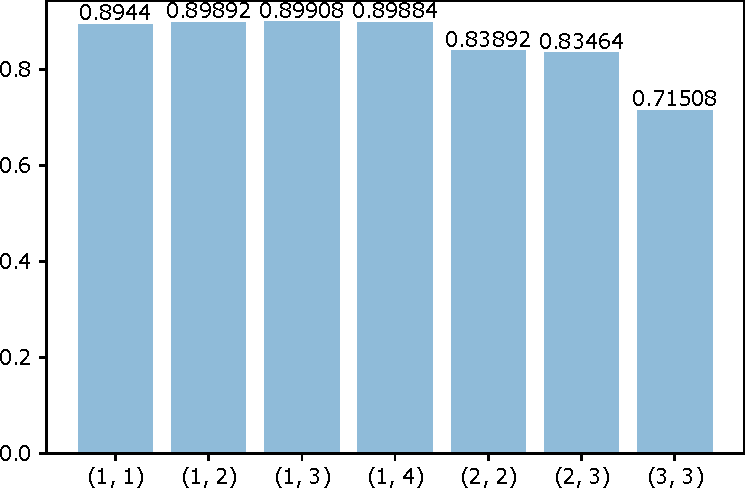
\includegraphics[scale=0.78]{grams.pdf}
\caption{Točnost klasifikatora u odnosu na izbor $n$-grama}
\end{figure}
\end{frame}

\begin{frame}
\frametitle{Nositelji sentimenta}
\begin{table}
    \center
    \begin{tabular}{| >{\bfseries}l | l | l | >{\bfseries}l | l | l |}
    \hline
    Rank & Leksem & Težina & Rank & Leksem & Težina\\ \hline
    1 & worst & -5.097 & 11 & fails & -2.966\\ \hline
    2 & 7/10 & 3.866 & 12 & great & 2.941\\ \hline
    3 & awful & -3.821 & 13 & disappointment & -2.933\\ \hline
    4 & bad & -3.495 & 14 & 8/ & 2.857\\ \hline
    5 & excellent & 3.456 & 15 & disappointing & -2.805\\ \hline
    6 & dull & -3.418 & 16 & poor & -2.788\\ \hline
    7 & waste & -3.413 & 17 & waste\_NEG & -2.779\\ \hline
    8 & 4/10 & -3.35 & 18 & 8 & 2.714\\ \hline
    9 & boring & -3.208 & 19 & unfortunately & -2.686\\ \hline
    10 & terrible & -3.04 & 20 & amazing & 2.67\\
    \hline
    \end{tabular}
    \caption{Nositelji sentimenta koji najviše utječu na klasifikaciju}
\end{table}
\end{frame}

\begin{frame}
\frametitle{Primjeri pogrešno klasificiranih primjeraka}
\begin{table}
\scalebox{0.80}{
    \begin{tabular}{| L{10 cm} | l | l |}
    \hline
    Isječak recenzije & Označeno & Klasificirano \\ \hline
    ...there's something compelling and memorable about it. 
    Like another commenter on the film, I saw this in childhood. 
    It's been thirty three years since 1952, but I have never forgotten the story or 
    its ridiculously cumbersome title. See it if you have the opportunity. & 0 & 1 \\  \hline
    ...HOWEVER, understand that the self-indulgent director also had many "funny gags" that 
    totally fell flat and hurt the movie. 
    His "camera tricks" weren't so much tricky but annoying and stupid. IGNORE THESE AND KEEP 
    WATCHING--it does get better. The film is fast paced, funny and worth seeing. In particular, 
    I really liked watching the acting and mugging of Max Linder--he was so expressive and funny! 
    Too bad he is virtually forgotten today. & 1 & 0\\
    \hline
    \end{tabular}}
\caption{Isječci pogrešno klasificiranih recenzija}
\end{table}
\end{frame}

\begin{frame}
\begin{center}
\Huge \textbf{DEMO}
\end{center}
\end{frame}

\begin{frame}
\begin{center}
\Huge Hvala na pažnji.
\end{center}
\end{frame}

\end{document}